% -- tau-transformations
%\newcommand{\smtxtit}[1]{\begin{scriptsize}\ensuremath{\textit{#1}}\end{scriptsize}}
\newcommand{\smtxtit}[1]{\ensuremath{\textit{#1}}}
\newcommand{\trans}[1]{\ensuremath{\tau_{#1}}\xspace}
\newcommand{\transtxt}[1]{\trans{\smtxtit{#1}}}
\def\transax{\transtxt{axioms}}
\def\transnorm{\transtxt{norm}}
\def\translt{\transtxt{lt}}
\def\transdlog{\transtxt{datalog}}

\def\LE{\ensuremath{\mathcal{L\!E}}\xspace}
\def\O{\ensuremath{\mathcal{O}}\xspace}
\def\P{\ensuremath{\mathcal{P}}\xspace}
\newcommand{\powset}[1]{\ensuremath{2^{#1}}\xspace}
\def\lprl{\ensuremath{\;:\!-\:}}
\def\cstr{\ensuremath{\;!-\:}}
\def\qury{\ensuremath{\;?-\:}}
\def\dlogrule{\lprl}
\def\dlogcstr{\square\lprl}
\def\dlogand{\wedge}
\def\dlognot{\sim}
\newcommand{\dlogfact}[1]{\ensuremath{{#1}\;.}}

% -- meta-level predicates
\newcommand{\predicate}[1]{\ensuremath{p_{#1}}\xspace}
\newcommand{\predsubtxt}[1]{\mathrm{\sf #1}}
\def\psco{\predicate{\predsubtxt{sco}}}
\def\pmo{\predicate{\predsubtxt{mo}}}
\def\phval{\predicate{\predsubtxt{hval}}}
\def\pitype{\predicate{\predsubtxt{itype}}}
\def\potype{\predicate{\predsubtxt{otype}}}
\def\mlaxioms{\ensuremath{P_{\smtxtit{meta}}}\xspace}

\newcommand{\typeof}{\ensuremath{typeOf}\xspace}

\section{Realizing WSML Reasoning through a Mapping to Datalog\label{sec:mapping}}
-- briefly sketch the idea of reasoning via rule based inferencing \\

The semantics of rule-based WSML is defined via a mapping to
datalog with (in)equality and integrity constraints. \sgr{probably
use a special denotation like $\textit{datalog}^{!=,IC}$, which
then has to be introduced in Section 2} To make use of existing
rule engines, the reasoning framework performs various
transformations to convert an original ontology in WSML syntax
into datalog rules. To maintain the semantics of more complex WSML
language constructs that cannot directly be expressed in datalog,
a fixed set of rules form the meta-level axioms that realise part
of the WSML semantics during reasoning. Based on the transformed
ontology, the WSML reasoning tasks of knowledge base
satisfiability and instance retrieval are realised by datalog
querying via calls to an underlying datalog inference engine that
is fed with the rules produced during transformation together with
the meta-level axioms.

\subsection{Transforming WSML to Datalog}
-- describe different transformation steps \\

The transformation of a WSML ontology to datalog rules forms a
pipeline of single transformation steps which are subsequently
applied, starting from the original ontology.

\paragraph{Axiomatization} -- In a first step, the transformation
\transax is applied as a mapping $\O \mapsto \powset{\LE}$ from
the set of all valid rule-based WSML ontologies to the powerset of
all logical expressions that conform to rule-based WSML. \transax
converts all conceptual syntax elements, such as concept and
attribute definitions or cardinality and type constraints, into
appropriate logical expressions according to
\cite{wsml-spec}(Table 8.1). \sgr{give the complete conversion
table instead of the following example ??}

To give an example, the WSML fragment
\begin{lstlisting}[style=wsml]
concept C subConceptOf D
    r ofType (0 2) T
instance a memberOf C
    r hasValue b,c
\end{lstlisting}
is translated by \transax to the following logical expressions.
\begin{lstlisting}[style=wsml]
C subConceptOf D. C[r ofType T]. !- ?x memberOf C and ?x[r
hasValue?y1, r hasValue ?y2] and ?y1 != ?y2. a memberOf C.  a
hasValue b,c.
\end{lstlisting}

\paragraph{Normalization} -- The transformation \transnorm is
applied to normalize WSML logical expressions as a mapping
$\powset{\LE} \mapsto \powset{\LE}$. This normalization step
reduces the complexity of WSML logical expressions according to
\cite{wsml-spec}(Section 8.2) to make them better fit the simple
syntactic form of literals in datalog rules. This reduction
includes conversion to negation and disjunctive normal forms as
well as decomposition of complex WSML molecules. The various
normalization steps are shown in Table \ref{tab:normalization}.
\sgr{include this table or rather skip it??} After \transnorm has
been applied, the resulting WSML logical expressions have the form
of logic programming rules with no deep nesting of logical
connectives.

\begin{table}[tb]\label{tab:normalization}\centering
\begin{footnotesize}
\begin{tabular}{|l|l|}
  \hline
  \rule{0cm}{3.2mm}{\normalsize \emph{original expression}} & {\normalsize \emph{normalized expression}} \\
  \hline
    $\transnorm(\{E_1 , \dots , E_n\})$ & $\{\transnorm(E_1) , \dots , \transnorm(E_n)\}$ \\
    $\transnorm(X$ \wsml{and} $Y.)$ & $\transnorm(X)$ \wsml{and} $\transnorm(Y)$ \\
    $\transnorm(X$ \wsml{or} $Y.)$ & $\transnorm(X)$ \wsml{or} $\transnorm(Y)$ \\
    $\transnorm(X$ \wsml{and} $(Y$ \wsml{or} $Z).)$ & $\transnorm(\transnorm(X)$ \wsml{and} $\transnorm(Y)$ \wsml{or} \\
    & $\phantom{\transnorm(}\transnorm(X)$ \wsml{and} $\transnorm(Z).)$ \\
    $\transnorm((X$ \wsml{or} $Y)$ \wsml{and} $Z).)$ & $\transnorm(\transnorm(X)$ \wsml{and} $\transnorm(Z)$ \wsml{or} \\
    & $\phantom{\transnorm(}\transnorm(Y)$ \wsml{and} $\transnorm(Z).)$ \\
    $\transnorm($ \wsml{naf} $ (X$ \wsml{and} $Y).)$ & $$ \wsml{naf} $ \transnorm(X)$ \wsml{or} $$ \wsml{naf} $ \transnorm(Y).$ \\
    $\transnorm($ \wsml{naf} $ (X$ \wsml{or} $Y).)$ & $$ \wsml{naf} $ \transnorm(X)$ \wsml{and} $$ \wsml{naf} $ \transnorm(Y).$ \\
    $\transnorm($ \wsml{naf} $ ($ \wsml{naf} $ X).)$ & $\transnorm(X)$ \\
    $\transnorm(X$ \wsml{implies} $Y.)$ & $\transnorm(Y)$\wsml{\lprl}$\transnorm(X).$ \\
    $\transnorm(X$ \wsml{impliedBy} $Y.)$ & $\transnorm(X)$\wsml{\lprl}$\transnorm(Y).$ \\
    $\transnorm(X[Y_1 , \dots , Y_n].)$ & $X[Y_1]$ \wsml{and} $\dots$ \wsml{and} $X[Y_n].$ \\
  \hline
\end{tabular}
\end{footnotesize}
\caption{Normalization of WSML logical expressions.}
\end{table}

\paragraph{Lloyd-Topor Transformation} -- The transformation
\translt is applied as a mapping $\powset{\LE} \mapsto
\powset{\LE}$ to flatten the complex WSML logical expressions,
producing simple rules according to the Lloyd-Topor
transformations \cite{lloyd-topor}, as shown in Table
\ref{tab:lloyd-topor}. \sgr{is the specification of the
lloyd-topor transformations correct? (esp. the middle one with
nested LP-rule and the lack of parenthesis)}
\begin{table}[tb]\label{tab:lloyd-topor}\centering
\begin{footnotesize}
\begin{tabular}{|l|l|}
  \hline
  \rule{0cm}{3.2mm}{\normalsize \emph{original expression}} & {\normalsize \emph{simplified rule(s)}} \\
  \hline
  $\translt(H_1$ \wsml{and} $\dots$ \wsml{and} $H_n$\wsml{\lprl}$B.)$ & $\translt(H_1$\wsml{\lprl}$B.)$ , \dots , $\translt(H_n$\wsml{\lprl}$B.)$ \\
  $\translt(H_1$\wsml{\lprl}$H_2$\wsml{\lprl}$B.)$ & $\translt(H_1$\wsml{\lprl}$H_2$ \wsml{and} $B.)$ \\
  $\translt(H$\wsml{\lprl} $B_1$ \wsml{or} , $\dots$ , \wsml{or} $B_n.)$ & $\translt(H$\wsml{\lprl}$B_1.)$ , \dots , $\translt(H$\wsml{\lprl}$B_n.)$ \\
  \hline
\end{tabular}
% --old tabel with Lloyd-Topor trasnformations
%\begin{tabular}{|c|c|}
%  \hline
%  % after \\: \hline or \cline{col1-col2} \cline{col3-col4} ...
%  \emph{original expression} & \emph{simplified rule(s)} \\
%  \hline
%  $H_1 \wedge \dots \wedge H_n \leftarrow B$ & $H_1 \leftarrow B , \dots , H_n \leftarrow B$ \\
%  $H_1 \leftarrow H_2 \leftarrow B$ & $H_1 \leftarrow H_2 \wedge B$ \\
%  $H \leftarrow B_1 \vee \dots \vee B_n$ & $H \leftarrow B_1 , \dots , H \leftarrow B_n$ \\
%  \hline
%\end{tabular}
\end{footnotesize}
\caption{Lloyd-Topor transformations.}
\end{table}
After this step, the resulting WSML expressions have the form of
proper datalog rules with a single head and conjunctive (possibly
negated) body literals.

\paragraph{Datalog Rule Generation} -- In a final step, the
transformation \transdlog is applied as a mapping $\powset{\LE}
\mapsto \P$ from all valid logical expressions in rule-based WSML
to the set of all datalog programs, yielding generic datalog rules
that represent the content of the original WSML ontology. In this
generic datalog program, all remaining WSML-specific language
constructs, such as \wsml{subConceptOf} or \wsml{ofType}, are
replaced by special meta-level predicates for which the semantics
of the respective language construct is encoded in meta-level
axioms as described in a further subsection.
\begin{table}[tb]\label{tab:LE2datalog}\centering
\begin{footnotesize}
\begin{tabular}{|l|l|}
  \hline
  \rule{0cm}{3.2mm} {\normalsize \emph{WSML}} & {\normalsize \emph{Datalog}} \\
  \hline
  $\transdlog(\{E_1, \dots , E_n\})$ & $\{\transdlog(E_1), \dots , \transdlog(E_n)\}$ \\
  $\transdlog($ \wsml{\cstr} $B.)$ & $\dlogcstr \transdlog(B)$ \\
  $\transdlog(H)$ & \dlogfact{\transdlog(H)} \\
  $\transdlog(H$ \wsml{\lprl} $B.)$ & $\transdlog(H) \dlogrule \transdlog(B)$ \\
  $\transdlog(X$ \wsml{and} $Y.)$ & $\transdlog(X) \dlogand \transdlog(Y)$ \\
  $\transdlog(C$ \wsml{subConceptOf} $D.)$ & $\psco(C,D)$ \\
  $\transdlog(I$ \wsml{memberOf} $C.)$ & $\pmo(I,C)$ \\
  $\transdlog(I[a$ \wsml{hasValue} $V].)$ & $\phval(I,a,V)$ \\
  $\transdlog(C[a$ \wsml{impliesType} $T].)$ & $\pitype(C,a,T)$ \\
  $\transdlog(C[a$ \wsml{ofType} $T].)$ & $\potype(C,a,T)$ \\
  $\transdlog($\wsml{r}$(X_1, \dots , X_n).)$ & $r(X_1, \dots , X_n)$ \\
  $\transdlog(X$ \wsml{=} $Y.)$ & $X = Y$ \\
  $\transdlog(X$ \wsml{!=} $Y.)$ & $X \neq Y$ \\
  \hline
\end{tabular}
\end{footnotesize}
\caption{Transformation from logical expressions in rule-based
WSML to datalog including meta-level predicates.}
\end{table}
Table \ref{tab:LE2datalog} shows the mapping from WSML logical
expressions to datalog including the meta-level predicates \psco,
\pmo, \phval, \pitype and \potype that represent their respective
WSML language constructs as can be seen from the mapping.

\bigskip

Ultimately, the basic\footnote{In Section \ref{sec:debugging} the
transformation pipeline is modified to support debugging
features.} transformation pipeline for converting a rule-based
WSML ontology into a datalog program is the following, constituted
by the single transformation steps introduced before.
\begin{displaymath}
    \tau = \transdlog \circ \translt \circ \transnorm \circ \transax
\end{displaymath}
As a mapping $\O \mapsto \P$, this chaining of the single steps is
applied to a WSML ontology $O \in \O$ to yield a semantically
equivalent datalog program $\tau (O) = P \in \P$ when interpreted
with respect to the meta-level axioms discussed next.

\subsection{WSML Semantics through Meta-Level Axioms}
\label{sec:meta}
%-- describe how a fixed set of rules implements (part of) the WSML semantics during reasoning \\
%-- -- each WSMl entity is mapped to a Datalog constant \\
%-- -- special meta-level predicates stand for specific WSMl constructs with a certain semantics; they are applied to Datalog constants (give example in picture) \\
%-- -- a direct mapping would not facilitate metamodelling as a feature of WSML \\
%-- -- meta-level axioms assure that the proper semantics of the wSMl constructs is maintained \\
%-- -- the meta-level axioms form rules for the meta-level predicates (, which appear in these rules) \\
%-- -- explain the intuition behind the various meta-level axioms \\

The mapping from WSML to Datalog in the reasoning framework works
such that each WSML-identifiable entity, i.e.\ concept, instance,
attribute etc., is mapped to an instance (or logical constant) in
Datalog, as depicted in Figure \ref{fig:meta}. There, the concepts
$C_1, C_2, C_3$ as well as the instances $I_1, I_2$ and the
attribute $a$ are mapped to constants such as $I_{C_1}$, $I_{I_1}$
or $I_a$ in Datalog, representing the original WSML entities on
the instance level.

Accordingly, the various special-purpose relations that hold
between WSML entities, such as \wsml{subConceptOf},
\wsml{memberOf} or \wsml{hasValue}, are mapped to Datalog
predicates that form a meta-level vocabulary for the WSML language
constructs. These are the meta-level predicates that appear in
Table \ref{tab:normalization} for \transdlog, and which are
applied to the Datalog constants that represent the WSML entities.
The facts listed in Figure \ref{fig:meta} illustrate the use of
the meta-level predicates. For example,
%
%the predicate \psco takes two Datalog constants as arguments that
%represent WSML concepts, to state that the concept represented by
%the first argument is a subconcept of the one represented by the
%second argument; on the other hand,
%
the predicate \pmo takes a Datalog constant that represents a WSML
instance and one that represents a WSML concept, to state that the
instance is in the extension of this concept.

In contrast to a direct mapping from WSML to Datalog with
concepts, attributes and instances mapping to unary predicates,
binary predicates and constants, respectively, this indirect
mapping allows for the WSML metamodelling facilities.
Metamodelling allows an entity to be a concept and an instance at
the same time. By representing a WSML entity as a Datalog
constant, it could, for example, fill both the first as well as
the second argument of e.g.\ the predicate \pmo.

\begin{figure}[tb]
\begin{minipage}[t]{6.5cm}
        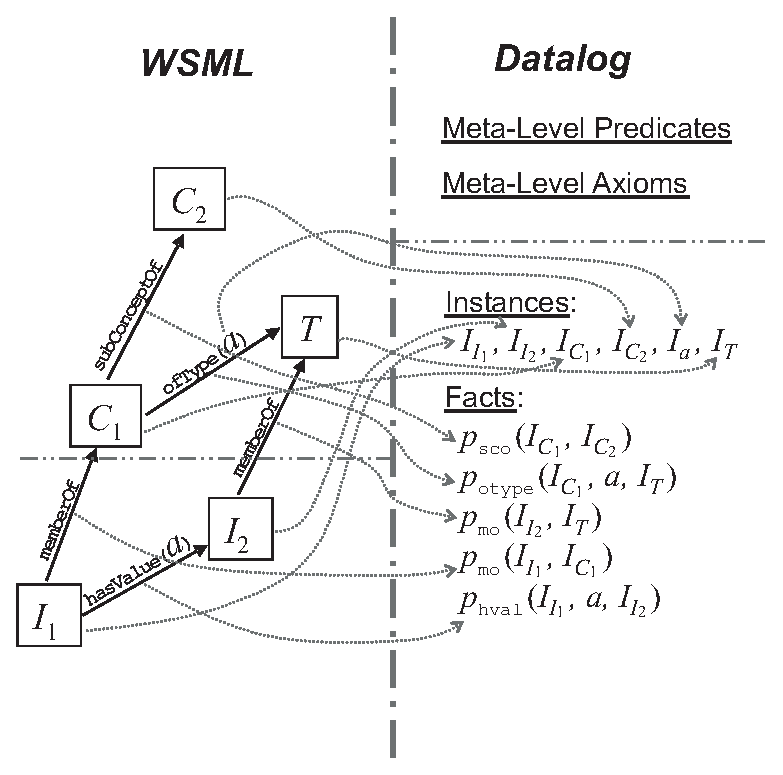
\includegraphics[width=6cm]{figures/meta}
        \raggedleft
\caption{Usage of meta-level predicates. \label{fig:meta}}
\end{minipage}\hfill
\begin{minipage}[t]{4.7cm}
\begin{small}
\vspace{-4.8cm}
\begin{tabular}{|ll|}
  \hline
  \multicolumn{2}{|l|}{\rule{0cm}{3.2mm}{\normalsize \emph{Meta-Level Axioms}}} \\
  \hline
  (1) & $\psco(C_1,C_3) \dlogrule \psco(C_1,C_2)$ \\
      & \phantom{$\psco(C_1,C_3) \dlogrule$} $\dlogand \psco(C_2,C_3)$ \\
  (2) & $\pmo(I,C_2) \dlogrule \pmo(I,C_1)$ \\
      & \phantom{$\pmo(I,C_2) \dlogrule$} $\dlogand \psco(C_1,C_2)$ \\
  (3) & $\pmo(V,C_2) \dlogrule \pitype(C_1,a,C_2)$ \\
      & \phantom{$\pmo(V,C_2) \dlogrule$} $\dlogand \pmo(I,C_1)$ \\
      & \phantom{$\pmo(V,C_2) \dlogrule$} $\dlogand \phval(I,a,V)$ \\
  (4) & $\dlogcstr \; \potype(C_1,a,C_2)$ \\
      & \phantom{$\dlogcstr \;$} $\dlogand \pmo(I,C_1)$ \\
      & \phantom{$\dlogcstr \;$} $\dlogand \phval(I,a,V)$ \\
      & \phantom{$\dlogcstr \;$} $\dlogand \dlognot \pmo(V,C_2)$ \\
 \hline
\end{tabular}
\caption{WSML semantics in Datalog. \label{tab:meta-level}}
\end{small}
\end{minipage}
\end{figure}

A fixed set \mlaxioms of Datalog rules, shown in
Figure~\ref{tab:meta-level}, forms the meta-level axioms which
assure that the original WSML semantics is properly maintained.
Axiom (1) realizes transitivity for the WSML \wsml{subConceptOf}
construct, while axiom (2) ensures that an instance of a
subconcept is also an instance of its superconcepts. Axiom (3)
realizes the semantics for the \wsml{implisType} construct for
attribute ranges: any attribute value is concluded to be in the
extension of the range type declared for the attribute. Finally,
axiom (4) realizes the semantics of the \wsml{ofType} construct by
a constraint that is violated whenever an attribute value cannot
be concluded to be in the extension of the declared range type.

\subsection{WSML Reasoning by Datalog Queries}
%-- describe how to realise WSML satisfiability and entailment through datalog querying \\
%-- -- characterize the KB (datalog program) on which reasoning is performed with the different facts and rules  \\
%-- -- show how the WSML reasoning tasks are mapped to datalog queries (KB sat., entailment and conjunctive query answering) \\

To perform reasoning over the original WSML ontology $O$ with an
underlying datalog inference engine, a datalog program
\begin{displaymath}
    P_O = \mlaxioms \cup \tau(O)
\end{displaymath}
is built up that consists of the meta-level axioms together with
the transformed ontology. The different WSML reasoning tasks are
then realized by performing Datalog queries on $P_O$. Posing a
query $Q(\vec{x})$ to a Datalog program $P \in \P$ is denoted by
$$(P,\qury Q(\vec{x}))$$ and yields a set of tuples that instantiate
the vector $\vec{x}$ of variables in the query.

\paragraph{Ontology Consistency} -- The task of checking a WMSL
ontology for consistency is done by querying for the empty clause,
as expressed by the following equivalence.
\begin{displaymath}
    O \; \textrm{\footnotesize{is satisfiable}} \; \Leftrightarrow \; (P_O , \qury \square) =
    \emptyset
\end{displaymath}
If the resulting set is empty then the empty clause could not be
derived from the program and the original ontology is satisfiable,
otherwise it is not.

\paragraph{Entailment} -- The reasoning task of entailment of
ground facts by a WSML ontology can be done by using queries that
contain no variables, as expressed in the following equivalence.
\begin{displaymath}
    O \models \phi \; \Leftrightarrow \; (P_O, \qury
    \tau'(\phi')) \not= \emptyset
\end{displaymath}
From the WSML ground fact $\phi \in \LE$ we derive a non-ground
formula $\phi' \in \LE$ by replacing the left-most occurrence of a
constant by the variable $x$. $\phi'$ is then transformed to
Datalog with a transformation $\tau' = \transdlog \circ \translt
\circ \transnorm$, similar to the one that is applied to the
ontology, and is evaluated together with the Datalog program
$P_O$. If the resulting set is non-empty then $\phi$ is entailed
by the original ontology, otherwise it is not.

\paragraph{Retrieval} -- Similarly, instance retrieval can be
performed by posing queries that contain variables to the Datalog
program $P_O$, as expressed in the following equivalence.
\begin{displaymath}
   % \{\vec{x} : O \models Q(\vec{x})\} \; \Leftrightarrow \; (P_O, \qury \tau(Q(\vec{x})))
   retrieve_O(Q) \; = \; (P_O, \qury \tau'(Q(\vec{x})))
\end{displaymath}
The query $Q(\vec{x})$, formulated as a WSML logical expression
with free variables $\vec{x}$, is transformed to Datalog and
evaluated together with the program $P_O$. The resulting set
contains all tuples $\vec{x}$ for which an instantiation of the
query expression is entailed by the original ontology.
To give an example, the query $Q($\syn{?x}$)$ = \\
\phantom{mmmmm} \syn{?x} \synkw{memberOf} \syn{BroadbandBundle}\\
posed to the ontology in Listing \ref{lst:wsml-ontology-example}
yields the set $\{ (\textit{MyBundle}) \}$ that contains one unary
tuple with the instance \textit{MyBundle}, which can be inferred
to be a broadband bundle due to its high network bandwidth.

%\begin{small}
%\begin{tabular}{|l|l|}
%  \hline
%  $O$ is satisfiable & $(P_O, \qury \dlognot \square) \rightarrow \top$ \\
%  $O \models \phi(\vec{C})$ & $(P_O, \qury \phi(\vec{C})) \rightarrow \top$ \\
%  $\{\vec{X} : O \models Q(\vec{X})\}$ & $\{\vec{X} : (P_O, \qury Q(\vec{X})) \rightarrow \top\}$ \\
% \hline
%\end{tabular}
%\end{small}
%
%( $\phi_g$ : ground fact ; $\vec{X}$ : variable binding )

\def\dataaxioms{\ensuremath{P_{\smtxtit{data}}}\xspace}
\def\transdpred{\transtxt{dpred}}

\subsection{Realising Datatype Reasoning}
\label{sec:datatype_reasoning} Although most of the generic
Datalog rules are understood by practically any Datalog
implementation, realizing datatype reasoning has some intricate
challenges. The main challenge is related to Axiom (4) in
Figure~\ref{tab:meta-level}, which checks attribute type
constraints. The crucial part of the axiom is the literal
\[\dlognot \pmo(V,C_2)\] because for datatype values no explicit
membership facts are included in the ontology that could
instantiate this literal. Consider, for example, the instance
\wsmlname{MSNDialup} from the WSML ontology in
Section~\ref{sec:wsml} -- there is no fact
$\pmo(10,\wsmlname{\_integer})$ for the value of the
\wsmlname{providesBandwidth} attribute. Whenever a value is
defined for an attribute constrained by \wsml{ofType}, Axiom (4)
would cause a constraint violation.

To solve this problem, \pmo facts should be generated for all
datatype constants that appear as values of attributes having
\wsml{ofType} constraints in the ontology. I.e., for each such
constant in the ontology, axioms of the following form should
appear: \compress
\begin{displaymath}
    \pmo(V,D) \lprl \typeof(V, D_T) \compress
\end{displaymath}
where $D$ denotes the WSML datatype, $D_T$ denotes a datatype
supported by the underlying Datalog implementation, which is
compatible with the WSML datatype, and \typeof denotes a built-in
predicate implemented by the Datalog tool, which checks whether a
constant value belongs to the specified datatype.

These additional meta-level axioms result in a new set of Datalog
rules, denoted by \dataaxioms, which are no longer in generic
Datalog but use tool-specific built-in predicates of the
underlying inference engine. The program $P_O$ is extended by
these rules as follows. \compress
\begin{displaymath}
    P_O = \mlaxioms \cup \dataaxioms \cup \tau(O)
\end{displaymath}

In addition to datatypes, WSML also supports some predefined
predicates on datatypes, such as numeric comparison
(see~\cite{wsml-spec} for a full list of WSML datatypes). The
definition of the axiom
\wsmlname{SharePriceFeed\_requires\_bandwidth} from the WSML
ontology in Section~\ref{sec:wsml}, for example, uses a shortcut of
the WSML \wsml{numericLessThan} predicate (denoted by $<$). For
translation of these special predicates to the corresponding
tool-specific built-in predicates supported by the underlying
Datalog reasoner, we introduce a new tool-specific transformation
step \transdpred as a mapping $\P \rightarrow \P$. This affects the
transformation pipeline $\tau$ as follows. \compress
\begin{displaymath}
    \tau = \transdpred \circ \transdlog \circ \translt \circ \transnorm \circ
    \transax \compress
\end{displaymath}

In summary, the underlying Datalog implementation must fulfill the
following requirements to support WSML datatype reasoning: (i) It
should provide built-in datatypes that correspond to WSML
datatypes. (ii) It should provide a predicate (or predicates) for
checking whether a datatype covers a constant and (iii) It should
provide built-in predicates that correspond to datatype-related
predefined predicates in WSML.

%\begin{itemize}
%    \item It should provide built-in datatypes that correspond to WSML datatypes.
%    \item It should provide a predicate (or predicates) for checking whether a datatype covers a constant.
%    \item It should provide built-in predicates that correspond to datatype-related predefined predicates in WSML.
%\end{itemize}

